\documentclass[tikz,border=8pt]{standalone}
% Shared look for every TikZ diagram. Load with \input{../../tools/tikz-style.tex}
\usepackage[T1]{fontenc}
\usepackage{lmodern}
\renewcommand{\sfdefault}{lmr}  % diagrams use the same serif as the text
\usetikzlibrary{arrows.meta, positioning, shapes.geometric, calc, fit, backgrounds}
\definecolor{cblue}{HTML}{4C78A8}
\definecolor{corange}{HTML}{F58518}
\definecolor{cgreen}{HTML}{54A24B}
\definecolor{cred}{HTML}{E45756}
\definecolor{cpurple}{HTML}{B279A2}
\definecolor{cgrey}{HTML}{6B6B6B}
\tikzset{
  every picture/.style={font=\sffamily, line width=1.2pt},
  box/.style={draw=#1, fill=#1!12, rounded corners=4pt, align=center, inner sep=7pt, minimum height=1.1cm},
  box/.default=cgrey,
  arrow/.style={-{Stealth[length=3mm]}, draw=cgrey, line width=1.4pt},
  title/.style={font=\sffamily\bfseries\Large},
  note/.style={font=\sffamily\small, text=cgrey, align=center},
}
\AtBeginDocument{\hyphenpenalty=10000 \exhyphenpenalty=10000}

\begin{document}
\begin{tikzpicture}[cell/.style={draw, thick, minimum size=1.7cm, font=\large}]
  \foreach \ox/\title/\hl in {0/Precision/col, 7/Recall/row} {
    \begin{scope}[xshift=\ox cm]
      \node[cell] (tn) at (0,0) {TN};
      \node[cell] (fp) at (1.7,0) {FP};
      \node[cell] (fn) at (0,-1.7) {FN};
      \node[cell] (tp) at (1.7,-1.7) {TP};
      \node[note, above=0.05cm of tn] {pred 0};
      \node[note, above=0.05cm of fp] {pred 1};
      \node[note, left=0.05cm of tn] {actual 0};
      \node[note, left=0.05cm of fn] {actual 1};
      \node[font=\bfseries\large, above=0.7cm of fp, xshift=-0.85cm] {\title};
    \end{scope}
  }
  % precision: column "pred 1"
  \draw[corange, line width=3pt, rounded corners] (0.82,0.88) rectangle (2.58,-2.58);
  \node[text=corange, align=center] at (1.0,-4.0) {$\dfrac{TP}{TP + FP}$\\[3pt] of everything \textbf{predicted} positive,\\ how much really is?};
  % recall: row "actual 1"
  \draw[cblue, line width=3pt, rounded corners] (6.12,-0.82) rectangle (9.58,-2.58);
  \node[text=cblue, align=center] at (8.0,-4.0) {$\dfrac{TP}{TP + FN}$\\[3pt] of everything \textbf{really} positive,\\ how much did we catch?};
\end{tikzpicture}
\end{document}
